\section{Introduction}
GPGPU (General-purpose computing on graphics processing units) has been on the rise, due to limitations for CPU's, such as power consumption, and the fact that the computational potential of GPU's (Graphical processing unit) is vastly greater than CPU's, see Figure \ref{potential}. There are technical/physical issue in reaching this potential, for example memory bandwidth, but there is also the conceptual issue of how to map parallelism to parallel hardware.
\begin{figure}[h]
	\centering
	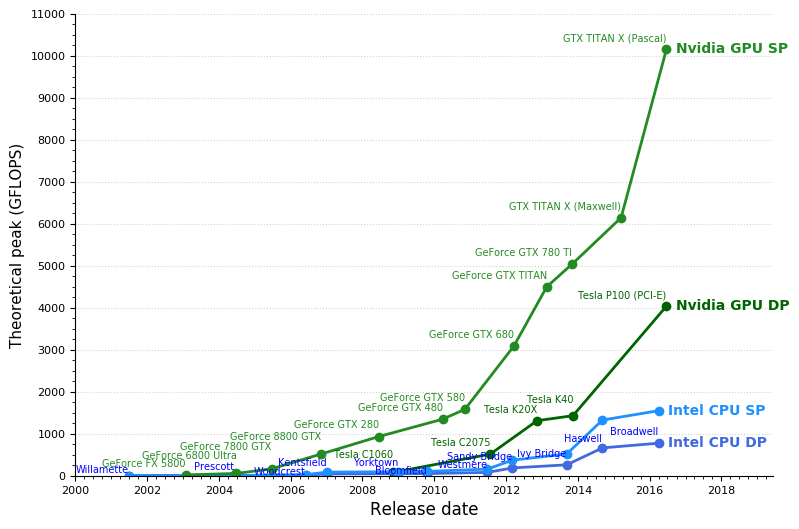
\includegraphics[width=.8\textwidth]{resources/graf.png}
	\caption{A graph showing the computational potential of CPUs and GPUs from 2000---2016 \cite{cpu-vs-gpu}}
	\label{potential}
\end{figure}

In this paper we will implement an autotuner for the programming language Futhark \cite{futhark-home}. Futhark is a statically typed, data-parallel, and purely functional array language, which support data-parallelism, and in-place array updates. The aim of Futhark is to shift the burden of writing efficient parallel code, from the programmer, to the compiler. The burden referred to is that to write efficient GPU code, a deep understanding of the hardware architecture, and the compiler is required. Not only does languages such as CUDA and OpenCL require this, but even when this knowledge is held it will result in non-portable code, since a lot of the optimizations made will be specific to a certain GPU, or at least to a certain GPU architecture. 

To achieve this shift the Futhark compiler creates multiple semantically equivalent versions of the code. These code versions will then exploit a different amount of parallelism.

In the following sections we will look at how Futhark solves the problem of
GPU's requiring flat parallelism, and the solution even being independent from
this limitation. An example of a simple problem, that is not flat, is the
\texttt{dotprod} function from listing \ref{matmultFuthark}. Here there is a \texttt{map2}\footnote{\texttt{map2} is a variant of \texttt{map} taking two arrays instead of a single element and an array. For example \texttt{map2 (+) [1,2,3] [4,5,6] $\to$ [5,7,9]}} which is nested inside of a \texttt{reduce}\footnote{Reduce does not obviously appear to be a parallel construct, due to the elements being dependent on each other, however this is done by a \textit{segmented reduce} \cite{segred}, making it effectively so.}, both operations are parallel, thereby giving \textit{nested parallelism}. In more general terms, nested parallelism is when there are parallel constructs nested within each other. Futhark supports such nested parallelism. More specifically, Futhark supports nested \textit{data}-parallelism. Data-parallelism is when some function/operation, is applied to a dataset in parallel, such that one thread uses function \texttt{x} on a subset of data \texttt{y}, and another thread also uses function \texttt{x}, but on a different subset of \texttt{y}. Other languages/environments that support nested data-parallelism are the likes of; CUDA, Open MP, OpenCL, NESL etc. With NESL being the conceptual precursor to the other languages. As mentoned earlier, NESL solved the issue of nested data-parallelism by flattening data structures (both regular and irregular), resulting in maximum parallelism, which can be inefficient. Therefore we need to determine when it is useful to exploit more parallelism. 

However mapping, effectively, functional code, to efficient parallel code, is difficult. Futhark does this by certain rules, these are conceptually similar to \textit{flattening} \cite{flat}, and is dubbed \textit{moderate flattening} \cite{futhark-nested-para}. While this approach was good, a pivotal element for achieving good performance in GPGPU, is to optimize for specific hardware, which moderate flattening did not do (neither does GPU languages such as CUDA or OpenCL, this is left to the programmer). To address this issue, the concept, and implementation, of \textit{incremental flattening} was developed. The concept is that Futhark will generate every distinct possible way of executing a program, these different executions are discriminated, at runtime, based on parameters passed to the program, these parameters symbolizes the amount of parallelism that the hardware executing the program possesses. The process of selection appropriate parameters, for the hardware, is called autotuning, which is what this paper implements.
